\documentclass[11pt]{article}
\usepackage{amssymb}
\usepackage{amsthm}
\usepackage{enumitem}
\usepackage{amsmath, physics}
\usepackage{bm}
\usepackage{adjustbox}
\usepackage{mathrsfs}
\usepackage{graphicx}
\usepackage{siunitx}
\usepackage[mathscr]{euscript}
\usepackage{tikz}
\usepackage{float}

\usetikzlibrary{automata, positioning, arrows}
\tikzset{
->, % makes the edges directed
>=stealth', % makes the arrow heads bold
node distance=3cm, % specifies the minimum distance between two nodes. Change if necessary.
every state/.style={thick, fill=gray!10}, % sets the properties for each ’state’ node
initial text=$ $, % sets the text that appears on the start arrow
}

\title{\textbf{Solved selected problems of Introduction to the Theory of Computation by Michael Sipser.}}
\author{Franco Zacco}
\date{}

\addtolength{\topmargin}{-3cm}
\addtolength{\textheight}{3cm}

\newcommand{\N}{\mathbb{N}}
\newcommand{\Z}{\mathbb{Z}}
\newcommand{\Q}{\mathbb{Q}}
\newcommand{\R}{\mathbb{R}}
\newcommand{\diam}{\text{diam}}
\newcommand{\cl}{\text{cl}}
\newcommand{\bdry}{\text{bdry}}
\newcommand{\inter}{\text{int}}
\newcommand{\hatx}{\bm{\hat{x}}}
\newcommand{\haty}{\bm{\hat{y}}}
\newcommand{\hatz}{\bm{\hat{z}}}
\newcommand{\hatrho}{\bm{\hat{\rho}}}
\newcommand{\hatphi}{\bm{\hat{\phi}}}
\newcommand{\hatr}{\bm{\hat{r}}}
\newcommand{\hattheta}{\bm{\hat{\theta}}}

\theoremstyle{definition}
% \newtheorem*{solution*}{Solution}
% \renewcommand*{\proofname}{\bf{Solution}}

\begin{document}
\maketitle
\thispagestyle{empty}

\section*{2 Context-Free Languages}
\subsection*{2.1 Context-Free Grammars}

\begin{proof}{\textbf{2.1}}
\begin{itemize}
    \item [\textbf{a.}] String: $a$ 
    \begin{figure}[H]
        \centering
        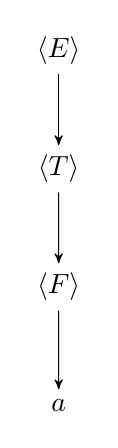
\begin{tikzpicture}
            \node{$\langle E \rangle$}
            child {node {$\langle T \rangle$}
                child {node {$\langle F \rangle$}
                    child {node {$a$}}
                }
            }
            ;
        \end{tikzpicture}    
    \end{figure}
    \item [\textbf{b.}] String: $a + a$ 
    \begin{figure}[H]
        \centering
        \begin{tikzpicture}
            \node{$\langle E \rangle$}
            child {node {$\langle E \rangle$}
                child {node {$\langle T \rangle$}
                    child {node {$\langle F \rangle$}
                        child {node {$a$}}
                    }
                }
            }
            child {node {$+$}}
            child {node {$\langle T \rangle$}
                child {node {$\langle F \rangle$}
                    child {node {$a$}}
                }
            }
            ;
        \end{tikzpicture}    
    \end{figure}
    \item [\textbf{c.}] String: $a + a + a$ 
    \begin{figure}[H]
        \centering
        \begin{tikzpicture}
            \node{$\langle E \rangle$}
            child {node {$\langle E \rangle$}
                child {node {$\langle E \rangle$}
                   child {node {$\langle T \rangle$}
                        child {node {$\langle F \rangle$}
                            child {node {$a$}}
                        }
                    }
                }
                child {node {$+$}}
                child {node {$\langle T \rangle$}
                    child {node {$\langle F \rangle$}
                        child {node {$a$}}
                    }
                }
            }
            child {node {$+$}}
            child {node {$\langle T \rangle$}
                child {node {$\langle F \rangle$}
                    child {node {$a$}}
                }
            }
            ;
        \end{tikzpicture}    
    \end{figure}
\cleardoublepage
    \item [\textbf{d.}] String: $((a))$ 
    \begin{figure}[H]
        \centering
        \begin{tikzpicture}
            \node{$\langle E \rangle$}
            child {node {$\langle T \rangle$}
                child {node {$\langle F \rangle$}
                    child {node {$($}}
                    child {node {$\langle E \rangle$}
                        child {node {$\langle T \rangle$}
                            child {node {$\langle F \rangle$}
                                child {node {$($}}
                                child {node {$\langle E \rangle$}
                                    child {node {$\langle T \rangle$}
                                        child {node {$\langle F \rangle$}
                                            child {node {$a$}}
                                        }
                                    }
                                }
                                child {node {$)$}}
                            }
                        }
                    }
                    child {node {$)$}}
                }
            }
            ;
        \end{tikzpicture}    
    \end{figure}
\end{itemize}
\end{proof}
\cleardoublepage
\begin{proof}{\textbf{2.2}}
\begin{itemize}
    \item [\textbf{a.}] Let us consider the intersection of languages $A$ and
    $B$ we see that $C = A \cap B$ contains the strings for the case $m = n$ so
    \begin{align*}
        a^mb^nc^n = a^nb^nc^m
    \end{align*}
    Then $C = \{a^nb^nc^n~|~n \geq 0\}$ but we saw in Example 2.36 that $C$ is
    not a context-free language. Therefore the class of context-free languages 
    is not closed under intersection.
    \item[\textbf{b.}] Let us consider the complement of the union of
    languages $A$ and $B$ i.e. $\overline{A \cup B}$ then by DeMorgan's law 
    we have that
    \begin{align*}
        \overline{A \cup B} = \overline{A}\cap\overline{B}
    \end{align*}
    But since the class of context-free languages is not closed under
    intersection then $\overline{A \cup B}$ might not be a context-free
    language. This implies that the class of context-free languages is not
    closed under complementation.
\end{itemize}
\end{proof}
\cleardoublepage
\begin{proof}{\textbf{2.3}}
\begin{itemize}
    \item [\textbf{a.}] The variables of $G$ are $R$, $S$, $T$ and $X$.
    \item [\textbf{b.}] The terminals of $G$ are $a$, $b$ and $\varepsilon$.
    \item [\textbf{c.}] The start variable of $G$ is $R$.
    \item [\textbf{d.}] $baa, ba$ and $aab$ are three strings in $L(G)$.
    \item [\textbf{e.}] $aaa, bbb$ and $\varepsilon$ are three strings not in
    $L(G)$.
    \item [\textbf{f.}] False because $T$ does not yield $aba$ but
    $XTX~|~X~|~\varepsilon$.
    \item [\textbf{g.}] True because
    $T \Rightarrow XTX \Rightarrow aTX \Rightarrow aTa \Rightarrow aXb
    \Rightarrow aba$.
    \item [\textbf{h.}] False because $T$ does not yield $T$ but
    $XTX~|~X~|~\varepsilon$.
    \item [\textbf{i.}] False because there are no finitely many steps such
    that $T$ can be derived into $T$.
    \item [\textbf{j.}] True because
    $XXX \Rightarrow aXX \Rightarrow abX \Rightarrow aba$.
    \item [\textbf{k.}] False because $X$ derives into $a~|~b$.
    \item [\textbf{l.}] True because
    $T \Rightarrow XTX \Rightarrow X\varepsilon X \Rightarrow XX$.
    \item [\textbf{m.}] True because
    $T \Rightarrow XTX \Rightarrow XXX$.
    \item [\textbf{n.}] False because $S \Rightarrow aTb~|~bTa$ and there is
    no way to remove the a's or b's after that.
    \item [\textbf{o.}] $L(G)$ is the language of strings which always
    contain $a$'s and $b$'s of length at least 2 i.e. $a$, $aa$, $bb$, $aaa$,
    $bbbb$, etc. are not in the language.
\end{itemize}
\end{proof}
\cleardoublepage
\begin{proof}{\textbf{2.4}}
    \begin{itemize}
        \item [\textbf{a.}] $\{w ~|~w \text{ contains at least three 1s}\}$
        \begin{align*}
            R_1 &\to 0R_1~|~1R_2\\
            R_2 &\to 0R_2~|~1R_3\\
            R_3 &\to 0R_3~|~1R_4\\
            R_4 &\to 0R_4~|~1R_4\\
            R_4 &\to \varepsilon
        \end{align*}
        \item [\textbf{b.}]
        $\{w ~|~w \text{ starts and ends with the same symbol}\}$
        \begin{align*}
            R_1 &\to 0R_20~|~1R_21\\
            R_2 &\to 0R_2~|~1R_2~|~\varepsilon
        \end{align*}
        \item [\textbf{c.}]
        $\{w ~|~\text{the length of $w$ is odd}\}$
        \begin{align*}
            R_1 &\to 0R_2~|~1R_2\\
            R_2 &\to 0R_1~|~1R_1~|~\varepsilon
        \end{align*}
        \item [\textbf{d.}]
        $\{w ~|~\text{the length of $w$ is odd and its middle symbol is a $0$}\}$
        \begin{align*}
            R_1 &\to 0R_10~|~0R_11~|~1R_10~|~1R_11~|~0
        \end{align*}
        \item [\textbf{e.}]
        $\{w ~|~w=w^R \text{, that is, $w$ is a palindrome}\}$
        \begin{align*}
            R_1 &\to 0R_10~|~1R_11~|~0~|~1
        \end{align*}
        \item [\textbf{f.}]
        The empty set.
        \begin{align*}
            R_1 &\to R_1
        \end{align*}
    \end{itemize}
\end{proof}
\cleardoublepage
\begin{proof}{\textbf{2.5}}
\begin{itemize}
    \item [\textbf{a.}] $\{w ~|~w \text{ contains at least three 1s}\}$
    \begin{figure}[H]
        \centering
        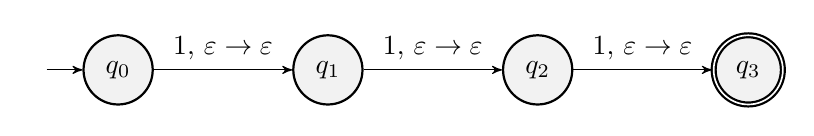
\begin{tikzpicture}
            \node[state, initial] (q0) {$q_0$};
            \node[state, right=5em of q0] (q1) {$q_1$};
            \node[state, right=5em of q1] (q2) {$q_2$};
            \node[state, right=5em of q2, accepting] (q3) {$q_3$};
            \draw
                (q0) edge[above] node{1, $\varepsilon \to \varepsilon$} (q1)
                (q1) edge[above] node{1, $\varepsilon \to \varepsilon$} (q2)
                (q2) edge[above] node{1, $\varepsilon \to \varepsilon$} (q3)
                ;
        \end{tikzpicture}    
    \end{figure}
    \item [\textbf{b.}]
    $\{w ~|~w \text{ starts and ends with the same symbol}\}$
    \begin{figure}[H]
        \centering
        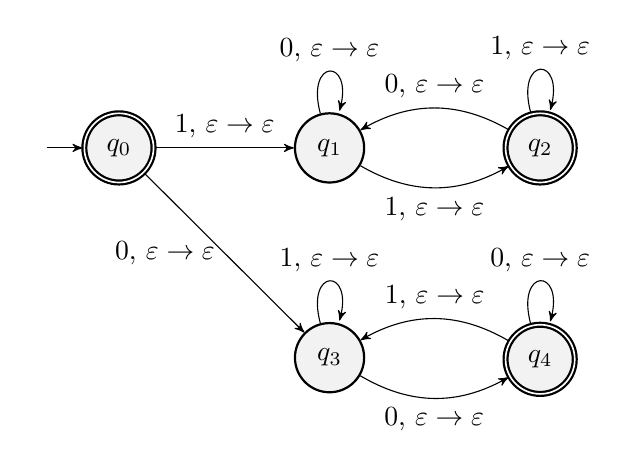
\begin{tikzpicture}
            \node[state, initial, accepting] (q0) {$q_0$};
            \node[state, right=5em of q0] (q1) {$q_1$};
            \node[state, right=5em of q1, accepting] (q2) {$q_2$};
            \node[state, below=5em of q1] (q3) {$q_3$};
            \node[state, below=5em of q2, accepting] (q4) {$q_4$};
            \draw
                (q0) edge[above] node{1, $\varepsilon \to \varepsilon$} (q1)
                (q1) edge[loop above] node{0, $\varepsilon \to \varepsilon$} (q1)
                (q1) edge[bend right, below] node{1, $\varepsilon \to \varepsilon$} (q2)
                (q2) edge[loop above] node{1, $\varepsilon \to \varepsilon$} (q2)
                (q2) edge[bend right,above] node{0, $\varepsilon \to \varepsilon$} (q1)

                (q0) edge[left] node{0, $\varepsilon \to \varepsilon$} (q3)
                (q3) edge[loop above] node{1, $\varepsilon \to \varepsilon$} (q3)
                (q3) edge[bend right, below] node{0, $\varepsilon \to \varepsilon$} (q4)
                (q4) edge[loop above] node{0, $\varepsilon \to \varepsilon$} (q3)
                (q4) edge[bend right,above] node{1, $\varepsilon \to \varepsilon$} (q3)
                ;
        \end{tikzpicture}
    \end{figure}
    \item [\textbf{c.}] $\{w ~|~\text{the length of $w$ is odd}\}$
    \begin{figure}[H]
        \centering
        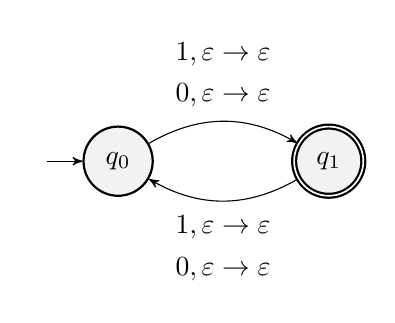
\begin{tikzpicture}
            \node[state, initial] (q0) {$q_0$};
            \node[state, right=5em of q0, accepting] (q1) {$q_1$};
            \draw
                (q0) edge[bend left, above] node{
                    $\begin{aligned}
                        1, \varepsilon \to \varepsilon\\
                        0, \varepsilon \to \varepsilon\\                        
                    \end{aligned}$
                } (q1)
                (q1) edge[bend left, below] node{
                    $\begin{aligned}
                        1, \varepsilon \to \varepsilon\\
                        0, \varepsilon \to \varepsilon\\                        
                    \end{aligned}$
                } (q0)
            ;
        \end{tikzpicture}
    \end{figure}
\cleardoublepage
    \item [\textbf{d.}]
    $\{w ~|~\text{the length of $w$ is odd and its middle symbol is a $0$}\}$
    \begin{figure}[H]
        \centering
        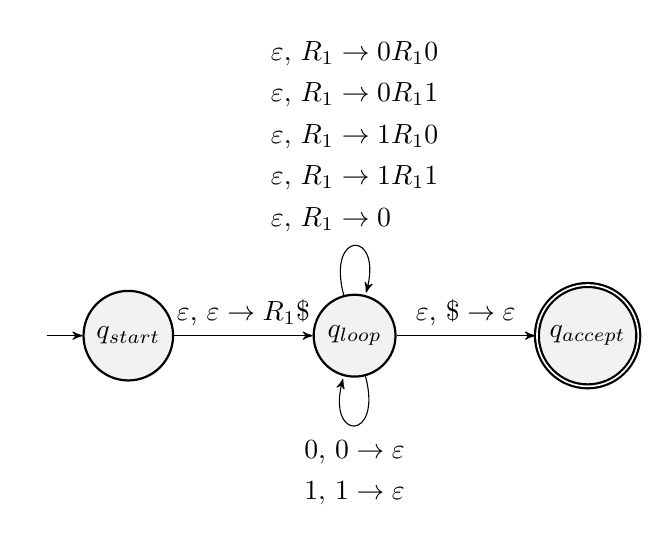
\begin{tikzpicture}
            \node[state, initial] (qstart) {$q_{start}$};
            \node[state, right=5em of qstart] (qloop) {$q_{loop}$};
            \node[state, right=5em of qloop, accepting] (qaccept) {$q_{accept}$};
            \draw
                (qstart) edge[above] node{$\varepsilon$, $\varepsilon \to R_1\$$} (qloop)
                (qloop) edge[loop above] node{
                    $\begin{aligned}
                        \varepsilon,~&R_1 \to 0R_1 0\\
                        \varepsilon,~&R_1 \to 0R_1 1\\
                        \varepsilon,~&R_1 \to 1R_1 0\\
                        \varepsilon,~&R_1 \to 1R_1 1\\
                        \varepsilon,~&R_1 \to 0
                    \end{aligned}$
                } (qloop)
                (qloop) edge[loop below] node{
                    $\begin{aligned}
                        0,~&0 \to \varepsilon\\
                        1,~&1 \to \varepsilon\\
                    \end{aligned}$
                } (qloop)
                (qloop) edge[above] node{$\varepsilon$, $\$ \to \varepsilon$} (qaccept)
            ;
        \end{tikzpicture}
    \end{figure}
    \item [\textbf{e.}] $\{w ~|~w=w^R \text{, that is, $w$ is a palindrome}\}$
    \begin{figure}[H]
        \centering
        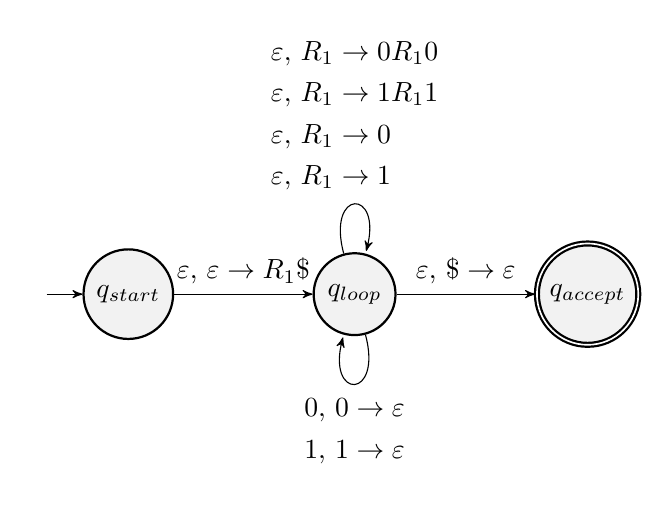
\begin{tikzpicture}
            \node[state, initial] (qstart) {$q_{start}$};
            \node[state, right=5em of qstart] (qloop) {$q_{loop}$};
            \node[state, right=5em of qloop, accepting] (qaccept) {$q_{accept}$};
            \draw
                (qstart) edge[above] node{$\varepsilon$, $\varepsilon \to R_1\$$} (qloop)
                (qloop) edge[loop above] node{
                    $\begin{aligned}
                        \varepsilon,~&R_1 \to 0R_1 0\\
                        \varepsilon,~&R_1 \to 1R_1 1\\
                        \varepsilon,~&R_1 \to 0\\
                        \varepsilon,~&R_1 \to 1
                    \end{aligned}$
                } (qloop)
                (qloop) edge[loop below] node{
                    $\begin{aligned}
                        0,~&0 \to \varepsilon\\
                        1,~&1 \to \varepsilon\\
                    \end{aligned}$
                } (qloop)
                (qloop) edge[above] node{$\varepsilon$, $\$ \to \varepsilon$} (qaccept)
            ;
        \end{tikzpicture}
    \end{figure}
    \item [\textbf{f.}] The empty set.
    \begin{figure}[H]
        \centering
        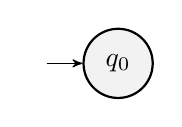
\begin{tikzpicture}
            \node[state, initial] (q0) {$q_{0}$};
            \draw
                (q0)
            ;
        \end{tikzpicture}
    \end{figure}
\end{itemize}
\end{proof}    
\cleardoublepage
\begin{proof}{\textbf{2.6}}
    \begin{itemize}
        \item [\textbf{a.}]
        The set of strings over the alphabet $\{a,b\}$ with more $a$'s than
        $b$'s
        \begin{align*}
            R_1 &\to bR_1a~|~aR_1b~|~baR_1~|~R_1ba~|~abR_1~|~R_1ab~|~R_2\\
            R_2 &\to R_1~|~a
        \end{align*}
        \item [\textbf{b.}]
        The complement of the language $\{a^nb^n~|~n\geq 0\}$
        \begin{align*}
            R_1 &\to bR_1a~|~baR_1~|~R_1ba~|~abR_1~|~R_1ab~|~R_2\\
            R_2 &\to R_1~|~a~|~b
        \end{align*}
        \item [\textbf{c.}]
        $\{w \# x~|~ w^R \text{ is a substring of $x$ for $w$}, x\in \{0,1\}^*\}$
        \begin{align*}
            R_0 &\to R_1R_2\\
            R_1 &\to 0R_10~|~1R_11~|~\# R_2\\
            R_2 &\to 0R_2~|~1R_2~|~\varepsilon
        \end{align*}
        \item [\textbf{d.}]
        $\{x_1 \# x_2\#...\# x_k ~|~ k \geq 1 \text{, each }x_i \in \{a,b\}^*,
        \text{ and for some $i$ and $j$, }x_i = x_j^R\}$
        \begin{align*}
            R_0 &\to R_1~|~R_2\#R_1\\
            R_1 &\to aR_1~|~bR_1~|~\#R_1~|~\varepsilon~|~R_0\\
            R_2 &\to aR_2a~|~bR_2b~|~\varepsilon~|~R_1
        \end{align*}
    \end{itemize}
\end{proof}
\cleardoublepage
\begin{proof}{\textbf{2.7}}
\begin{itemize}
    \item [\textbf{a.}]
    The set of strings over the alphabet $\{a,b\}$ with more $a$'s than
    $b$'s

    The PDA for this language should do as follows, we read the first symbol,
    suppose it's an $a$ then we push it to the stack, then we read the next
    symbol if it's a $b$ we pop the stack, if it's another $a$ we push it
    to the stack. If the first symbol was a $b$ and the next one is an $a$
    then we pop the $b$ and so on. We continue this process until we read the
    entire input. If we only have $a$'s in the stack, we accept it; otherwise,
    we reject it.

    \item [\textbf{b.}]
    The complement of the language $\{a^nb^n~|~n\geq 0\}$

    The PDA for this language should do as follows.\\
    If the first input symbol is a $b$ we accept.\\
    If the first input string is a set of $a$'s we push them to the stack
    and if the next symbols are $b$'s we pop the stack for each one of them
    to check if we have the same number of $a$'s. If that's the case, we reject
    otherwise, we accept.\\
    If after any number of $a$'s and $b$'s we still read another $a$ we accept.

    \item [\textbf{c.}]
    $\{w \# x~|~ w^R \text{ is a substring of $x$ for $w$}, x\in \{0,1\}^*\}$

    The PDA for this language should do as follows.\\
    We read each symbol and we push it to the stack until we read a $\#$,
    if there is no $\#$ we reject. Then non-deterministically we read the
    subsequent symbols and check if they match to the ones in the stack,
    if they match, we pop them from the stack. If the stack is empty in any of
    the non-deterministic branches when we finish reading the input we accept.
    Otherwise we reject.    

    \item [\textbf{d.}]
    $\{x_1 \# x_2\#...\# x_k ~|~ k \geq 1 \text{, each }x_i \in \{a,b\}^*,
    \text{ and for some $i$ and $j$, }x_i = x_j^R\}$

    The PDA for this language should do as follows.\\
    Suppose $x_2 = x_1^R$, then we read each symbol of $x_1$ and we push it to
    the stack until we read a $\#$ then we read $x_2$ and we pop the symbols
    that match with the ones we have on the stack since $x_2 = x_1^R$.\\
    Now suppose $x_j = x_1^R$ then we do the same but non-deterministically,
    we check each $x_j$ with the process mentioned in the previous paragraph.\\
    Finally, if $x_1$ is not the string reversed, then we have to check
    non-deterministically every $x_i$ as we did before to check which one is
    the one reversed. In each non-deterministic branch, we store $x_i$ in the
    sack, and we check as in the previous paragraph which $x_j$ matches to
    $x_i^R$.\\
    In the case the input has no $\#$ or no string matches to another reversed
    string we reject.
\end{itemize}
\end{proof}
\cleardoublepage
\begin{proof}{\textbf{2.8}}
    One leftmost derivation of "the girl touches the boy with the flower" in
    grammar $G_2$ is
    \begin{align*}
        \langle SENTENCE \rangle
        &\Rightarrow \langle NOUN-PHRASE \rangle\langle VERB-PHRASE \rangle\\
        &\Rightarrow \langle CMPLX-NOUN \rangle\langle VERB-PHRASE \rangle\\
        &\Rightarrow \langle ARTICLE \rangle\langle NOUN \rangle
        \langle VERB-PHRASE \rangle\\
        &\Rightarrow \text{the }\langle NOUN \rangle\langle VERB-PHRASE \rangle\\
        &\Rightarrow \text{the girl }\langle VERB-PHRASE \rangle\\
        &\Rightarrow \text{the girl }\langle CMPLX-VERB \rangle\\
        &\Rightarrow \text{the girl }\langle VERB \rangle
        \langle NOUN-PHRASE \rangle\\
        &\Rightarrow \text{the girl touches }\langle NOUN-PHRASE \rangle\\
        &\Rightarrow \text{the girl touches }
        \langle CMPLX-NOUN \rangle\langle PREP-PHRASE \rangle\\
        &\Rightarrow \text{the girl touches }\langle ARTICLE \rangle
        \langle NOUN \rangle\langle PREP-PHRASE \rangle\\
        &\Rightarrow \text{the girl touches the }
        \langle NOUN \rangle\langle PREP-PHRASE \rangle\\
        &\Rightarrow \text{the girl touches the boy }
        \langle PREP-PHRASE \rangle\\
        &\Rightarrow \text{the girl touches the boy }
        \langle PREP \rangle\langle CMPLX-NOUN \rangle\\
        &\Rightarrow \text{the girl touches the boy with }
        \langle CMPLX-NOUN \rangle\\
        &\Rightarrow \text{the girl touches the boy with }
        \langle ARTICLE \rangle\langle NOUN \rangle\\
        &\Rightarrow \text{the girl touches the boy with the }
        \langle NOUN \rangle\\
        &\Rightarrow \text{the girl touches the boy with the flower}
    \end{align*}
    But we also have the following leftmost derivation of this phrase
    \begin{align*}
        \langle SENTENCE \rangle
        &\Rightarrow \langle NOUN-PHRASE \rangle\langle VERB-PHRASE \rangle\\
        &\Rightarrow \langle CMPLX-NOUN \rangle\langle VERB-PHRASE \rangle\\
        &\Rightarrow \langle ARTICLE \rangle\langle NOUN \rangle
        \langle VERB-PHRASE \rangle\\
        &\Rightarrow \text{the }\langle NOUN \rangle\langle VERB-PHRASE \rangle\\
        &\Rightarrow \text{the girl }\langle VERB-PHRASE \rangle\\
        &\Rightarrow \text{the girl }\langle CMPLX-VERB \rangle
        \langle PREP-PHRASE \rangle\\
        &\Rightarrow \text{the girl }\langle VERB \rangle
        \langle NOUN-PHRASE\rangle\langle PREP-PHRASE \rangle\\
        &\Rightarrow \text{the girl touches }\langle NOUN-PHRASE\rangle
        \langle PREP-PHRASE \rangle\\
        &\Rightarrow \text{the girl touches }\langle CMPLX-NOUN\rangle
        \langle PREP-PHRASE \rangle\\
        &\Rightarrow \text{the girl touches }\langle ARTICLE\rangle
        \langle NOUN\rangle\langle PREP-PHRASE \rangle\\
        &\Rightarrow \text{the girl touches the }
        \langle NOUN\rangle\langle PREP-PHRASE \rangle\\
        &\Rightarrow \text{the girl touches the boy }
        \langle PREP-PHRASE \rangle\\
        &\Rightarrow \text{the girl touches the boy }
        \langle PREP\rangle\langle CMPLX-NOUN\rangle\\
        &\Rightarrow \text{the girl touches the boy with }
        \langle CMPLX-NOUN\rangle\\
        &\Rightarrow \text{the girl touches the boy with }
        \langle ARTICLE\rangle\langle NOUN\rangle\\
        &\Rightarrow \text{the girl touches the boy with the }
        \langle NOUN\rangle\\
        &\Rightarrow \text{the girl touches the boy with the flower}
    \end{align*}
\end{proof}
\cleardoublepage
\begin{proof}{\textbf{2.13}}
\begin{itemize}
    \item [\textbf{a.}] $L(G)$ describes strings with two $\#$s
    betwen a number of $0$s including no $0$s i.e. two $\#$ between an even
    number of $0$s.

    Also, $L(G)$ describes strings starting with $n$-zeros a $\#$ and ending
    with twice as many zeros ($2n$ zeros).
    \item [\textbf{b.}] Suppose $L(G)$ is a regular language, we want to arrive
    at a contradiction.
    
    Let $s = 0^p\#0^{2p}$ we see that $s \in L(G)$ then by the
    pumping lemma $s$ can be divided into three pieces $s = xyz$ such that
    $|y| > 0$ and $|xy| \leq p$ but also has to be that $xy^iz \in L(G)$
    for each $i \geq 0$.

    Because we need that $|xy| \leq p$ then the only way we can divide $s$
    is as follows.

    Let $0 \leq j < k \leq p$ and let us divide $s$ as
    \begin{align*}
        \underbrace{0^j}_x\underbrace{0^k}_y\underbrace{0^{p - k}\#0^{2p}}_z
    \end{align*}
    We see that $|y| > 0$ and $|xy| \leq p$ as desired.  Now, if we take $i = 2$
    should be that $0^j0^{2k}0^{p-k}\#0^{2p}$ is in $L(G)$ but for this to
    happen must be that 
    \begin{align*}
        2(j + 2k + (p-k)) &= 2p\\
        2j + 2k &= 0\\
        k &= -j
    \end{align*}
    Which cannot happen and hence $s$ does not comply with the pumping lemma.

    Therefore we have arrived at a contradiction and must be that $L(G)$ is
    not regular.
\end{itemize}
\end{proof}
\cleardoublepage
\begin{proof}{\textbf{2.16}}
    Let $L(G_1)$ and $L(G_2)$ be context-free languages generated by the
    context-free grammars $G_1 = (V_1, \Sigma, R_1, S_1)$ and
    $G_2 = (V_2, \Sigma, R_2, S_2)$ then we can construct 
    $$G_U = (V_1 \cup V_2 \cup \{S\}, \Sigma, R_1 \cup R_2 \cup \{r\}, S)$$
    where $r$ sets the new start variable such that $S \to S_1~|~S_2$.
    Then $L(G_U) = L(G_1) \cup L(G_2)$ and hence the context-free languages are
    closed under the union operation.

    Now, let us contruct
    $$G_\circ = (V_1 \cup V_2 \cup \{S\}, \Sigma, R_1 \cup R_2 \cup \{r\}, S)$$
    but in this case we define $r$ as $S \to S_1S_2$ so
    $L(G_\circ) = L(G_1) \cap L(G_2)$ and hence the context-free languages are
    closed under the concatenation operation.

    Finally, we construct
    $$G_* = (V_1 \cup \{S\}, \Sigma, R_1 \cup \{r\}, S)$$
    where in this case we define $r$ as $S \to SS_1 | \varepsilon$ so
    $L(G_*) = L(G_1)^*$ and hence the context-free languages are
    closed under the star operation.
\end{proof}

\cleardoublepage
\begin{proof}{\textbf{2.17}}
Let $R$ be a regular expression, then $R$ is 
\begin{itemize}
    \item [\textbf{1.}] $a$ for some $a$ in the alphabet $\Sigma$
    \item [\textbf{2.}] $\varepsilon$
    \item [\textbf{3.}] $\emptyset$
    \item [\textbf{4.}] $R_1 \cup R_2$ where $R_1$ and $R_2$ are regular expressions
    \item [\textbf{5.}] $R_1 \circ R_2$ where $R_1$ and $R_2$ are regular expressions
    \item [\textbf{6.}] $R_1^*$ where $R_1$ is a regular expression
\end{itemize}
Then if $R = a$ we can define a context-free grammar $G$ such that
$$S \to a$$
Which recognizes $a$.
If $R = \varepsilon$ then we define $G$ as
$$S \to \varepsilon$$
And if $R = \emptyset$ then we define $G$ as
$$S \to S$$
In any of the rest of the cases, context-free languages are closed under union,
concatenation, and star operation, so we can always find a context-free grammar
that is equivalent to the regular expression $R$.
Therefore, every regular language is context-free.
\end{proof}

\cleardoublepage
\begin{proof}{\textbf{2.30}}
\begin{itemize}
    \item [\textbf{a.}] Let $A = \{0^n1^n0^n1^n~|~n\geq0\}$, we want to show 
    that $A$ is not context free by contradiction, so let us assume
    that $A$ is context-free.

    Let us select a string $s = 0^p1^p0^p1^p$ which is a member of $A$ and
    of length at least $p$, then $s$ can be divided into $s = uvxyz$.

    Condition 2 stipulates that either $v$ or $y$ is nonempty. Then we consider
    two cases.
    \begin{itemize}
        \item [1.] Suppose $v$ and $y$ contains only one type of alphabet
        symbol, then pumping $s$ to $uv^2xy^2z$ will have different number
        of $0$s and/or $1$s in the string and so $uv^2xy^2z$ will not be in
        $A$. Hence we have a contradiction.
        
        \item [2.] When either $v$ or $y$ contain more than one type of symbol
        then $uv^2xy^2z$ may contain equal numbers of 0s and 1s but not in the
        correct order. Hence we have another contradiction.
    \end{itemize}
    Because both cases result in a contradiction, a contradiction is
    unavoidable. Therefore $A$ is not context free.

    \item [\textbf{b.}] Let $A = \{0^n\#0^{2n}\#0^{3n}~|~n\geq0\}$, we want to
    show  that $A$ is not context free by contradiction, so let us assume
    that $A$ is context-free.

    Let us select a string $s = 0^p\#0^{2p}\#0^{3p}$ which is a member of $A$ and
    of length at least $p$, then $s$ can be divided into $s = uvxyz$.

    Condition 2 stipulates that either $v$ or $y$ is nonempty. Then we consider
    two cases.
    \begin{itemize}
        \item [1.] Suppose $v$ and $y$ contains only one type of alphabet
        symbol, then pumping $s$ to $uv^2xy^2z$ creates a string which either
        has two $\#$s if $v$ or $y$ equals to $\#$ or we have a string that
        doesn't match the expected form i.e. has more $0$s in one part of the
        string, so the lengths $n, 2n, 3n$ of each substring is not maintained.
        Hence we have a contradiction.
        
        \item [2.] When either $v$ or $y$ contain more than one type of symbol
        then $uv^2xy^2z$ creates a string with two $\#$ and so 
        $uv^2xy^2z$ is not in $A$. Hence we have another contradiction.
    \end{itemize}
    Because both cases result in a contradiction, a contradiction is
    unavoidable. Therefore $A$ is not context free.

\cleardoublepage
    \item [\textbf{c.}]
    Let $A = \{w\#t~|~w \text{ is a substring of $t$, where } w,t \in \{a,b\}^*\}$
    we want to show  that $A$ is not context free by contradiction, so let us
    assume that $A$ is context-free.

    Let us select the string $s = a^pb^p\#a^pb^p$ which is a member of $A$ and
    of length at least $p$, then $s$ can be divided into $s = uvxyz$.

    Condition 2 stipulates that either $v$ or $y$ is nonempty. Then we consider
    two cases.
    \begin{itemize}
        \item [1.] Suppose $v$ and $y$ contains only one type of alphabet
        symbol and not $\#$, then three cases can happen
        \begin{itemize}
            \item [i.] If $v$ and $y$ are on the left side of the string
            (to the left of the $\#$) then the left side of the pumped string
            $uv^2xy^2z$ is not a substring of the right side of the string.
            A contradiction.
            \item [ii.] If $v$ and $y$ are on the right side of the string
            then the "down pumped" string $uv^0xy^0z$ creates a string into
            which the left side is not a substring of the right side.
            A contradiction.
            \item [iii.] Finally, if $v$ is on the left side and $y$ is on the
            right side then $v$ has to be formed by some number of $b$'s and
            $y$ has to be some number of $a$'s, otherwise, we have that
            $|vxy| > p$. Then the pumped string $uv^2xy^2z$ is not in $A$ since
            the left side is not a substring of the right side
            (it has more $b$'s). A contradiction.
        \end{itemize}

        \item [2.] When either $v$ or $y$ contain more than one type of symbol
        then two cases can happen
        \begin{itemize}
            \item [i.] If $v$ and $y$ are on the left side of the string then
            the pumped string $uv^2xy^2z$ is not in $A$ because the left side
            of the string is not a substring of the right side.
            A contradiction.
            \item [i.] If $v$ and $y$ are on the right side of the string then
            the "down pumped" string $uv^0xy^0z$ is not in $A$ since the left
            side is not a substring of the right side.
            A contradiction.
        \end{itemize}
    \end{itemize}
    Because all cases result in a contradiction, a contradiction is unavoidable.
    Therefore $A$ is not context free.

\cleardoublepage
    \item [\textbf{d.}]
    Let $$A = \{t_1 \# t_2 \# ... \# t_k ~|~k\geq 2,
    \text{ each } t_i \in \{a,b\}^*, \text{ and } t_i = t_j \text{ for some }
    i \neq j \}$$
    we want to show  that $A$ is not context free by contradiction, so let us
    assume that $A$ is context-free.

    Let $t_1 = t_2 = a^pb^p$ then the string $s = a^pb^p\#a^pb^p$ is in $A$ and
    of length at least $p$, then $s$ can be divided into $s = uvxyz$.

    As we showed before if $v$ and $y$ are on the left side of the string 
    (left to the $\#$) then the left side of $uv^2xy^2z$ is going to be
    different from the right side and hence $t_1 \neq t_2$.

    The same can be shown for $v$ and $y$ on the right side of the string.

    So the only option left is that $v$ is on the left side and $y$ is on the
    right side but then $v$ has to be formed by some number of $b$'s and
    $y$ has to be some number of $a$'s, otherwise, we have that $|vxy| > p$.

    Then the pumped string $uv^2xy^2z$ is not in $A$ since the left side is
    not equal the right side.

    Therefore in any case we get a contradiction and hence $A$ is not context
    free.
\end{itemize}
\end{proof}
\end{document}
